\section{Step 1: Geometry}
\label{sec:geometry}

The flow domain is a flat rectangle in the $xy$ plane, above the rocket axis ($y \geq 0$), with the
outline of the nose cut out of its lower edge (Figure~\ref{fig:domain}). It is built in Discovery, inside
Workbench, from the design STEP file.

\subsection{Steps}

\begin{enumerate}
\item \textbf{Workbench.} Add a \gui{Fluid Flow (Fluent)} system. Before importing anything, click the
\gui{Geometry} cell and set \gui{Properties}\then\gui{Analysis Type} = \gui{2D}. Without this setting,
Fluent does not offer the axisymmetric option used below.
\item \textbf{Import.} \gui{Geometry}\then\gui{Import Geometry}\then\gui{Browse}, choose
\file{CFD/geometry_650/nose_lvhaack_L561_c89_rn4.5mm.step} and open it in \gui{Discovery}
(Figure~\ref{fig:geom-step}). Use the STEP file, not the STL: the STL is made of small flat triangles,
and cutting, naming edges and meshing do not work cleanly on it.
\item \textbf{Extend the body.} With \gui{Pull}, drag the flat end face of the coupler by
\SI{+1800}{mm}, from $x = \SI{647.65}{mm}$ to $x = \SI{2447.65}{mm}$. The body is now a long cylinder
that reaches the end of the domain.
\item \textbf{Draw the domain.} In the $XY$ plane, sketch the rectangle from $x = -3600$, $y = 0$ to
$x = 2447.65$, $y = 3600$ (mm) and turn it into a surface.
\item \textbf{Cut out the body.} \gui{Combine}\then\gui{Subtract from target}: the rectangle is the
target, the solid is the tool that cuts. Delete the solid and any piece left inside the body. One
surface remains, with the half-outline of the nose along its lower edge (Figure~\ref{fig:geom-domain}).
The nose and cylinder edges are already separate, because they are separate faces in the STEP file.
\item \textbf{Save the project} (\gui{File}\then\gui{Save As}). Until it is saved, Workbench keeps the
geometry in a temporary folder and loses it if it restarts. The study-A domain is stored as
\file{CFD/geometry_650/studyA_domain2D_2024R2.dsco}.
\item \textbf{Name the edges.} In Meshing, select each edge, right-click\then\gui{Create Named
Selection}, and use exactly the names of Table~\ref{tab:named}. Fluent turns them into boundaries with
the same names, and the boundary conditions of Step~3 are set on them (Figure~\ref{fig:geom-named}). A
typing error (\zone{wal\_nose}) means renaming the zone in Fluent later.
\end{enumerate}

\begin{table}[H]
\centering
\caption{Named edges of the study-A domain (Figure~\ref{fig:domain}).}
\label{tab:named}
\small
\begin{tabular}{@{}lll@{}}
\toprule
Name & Edge & Position [m] \\
\midrule
\zone{inlet} & left (upstream) edge & $x = -3.6$, $y$ from 0 to 3.6 \\
\zone{farfield} & top edge & $y = 3.6$, $x$ from $-3.6$ to 2.44765 \\
\zone{outlet} & right (downstream) edge & $x = 2.44765$, $y$ from 0.09 to 3.6 \\
\zone{axis} & rocket axis in front of the tip & $y = 0$, $x$ from $-3.6$ to 0 \\
\zone{wall\_nose} & curved nose, rounded tip included & $x$ from 0 to 0.55865 \\
\zone{wall\_body} & cylinder: coupler and its extension & $y = 0.09$, $x$ from 0.55865 to 2.44765 \\
\bottomrule
\end{tabular}
\end{table}

\checkstep{The surface lies entirely above the axis ($y \geq 0$), the $x$ axis is the rocket axis, the
tip is at the origin, and every edge has exactly one name. When the mesh is read into Fluent, the console
lists one fluid zone and these six boundaries.}

\subsection{Why the domain looks like this}

\begin{figure}[H]
\centering
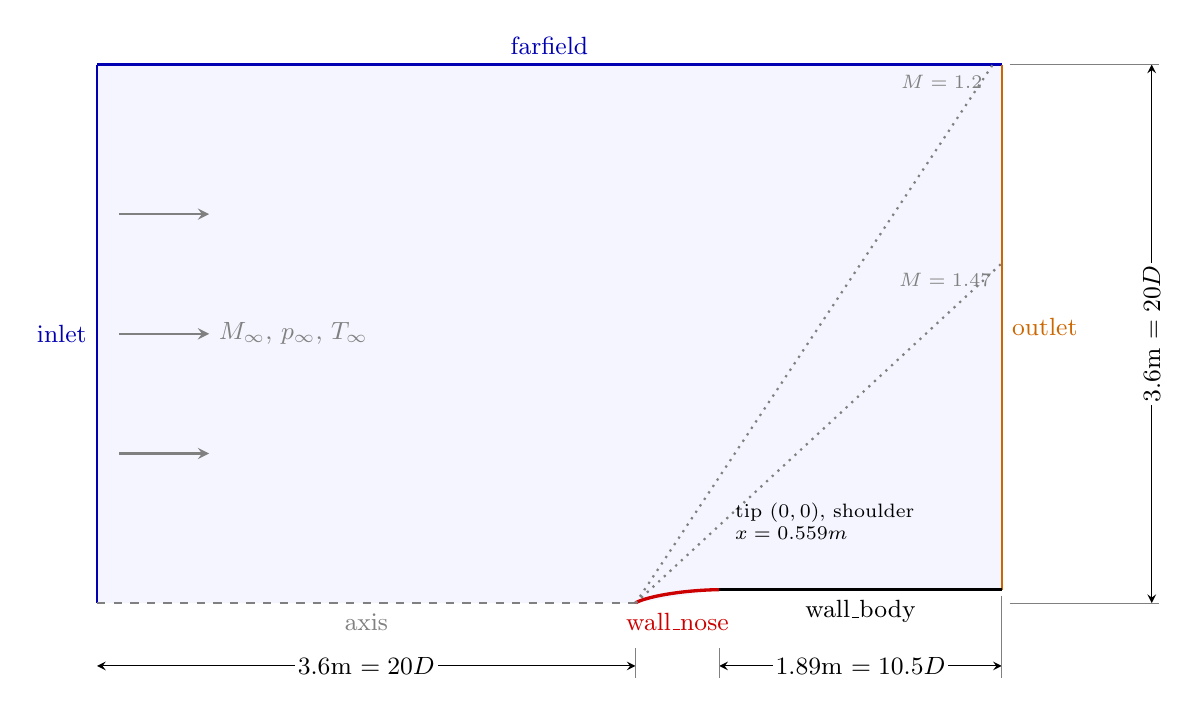
\begin{tikzpicture}[x=1.9cm,y=1.9cm,>=stealth,font=\small]
  % domain, to scale (x from -3.6 to 2.448 m, y from 0 to 3.6 m)
  \fill[blue!4] (-3.6,0) -- (0,0) -- (0.559,0.09) -- (2.448,0.09) -- (2.448,3.6) -- (-3.6,3.6) -- cycle;
  \draw[thick,blue!70!black] (-3.6,0) -- (-3.6,3.6) node[midway,left,align=right] {\zone{inlet}};
  \draw[thick,blue!70!black] (-3.6,3.6) -- (2.448,3.6) node[midway,above] {\zone{farfield}};
  \draw[thick,orange!80!black] (2.448,0.09) -- (2.448,3.6) node[midway,right] {\zone{outlet}};
  \draw[thick,dashed,gray] (-3.6,0) -- (0,0) node[midway,below] {\zone{axis}};
  \draw[very thick,red!80!black] plot[domain=0:180,samples=40,variable=\t]
     ({0.559*(1-cos(\t))/2},{0.09/sqrt(pi)*sqrt(rad(\t)-sin(2*\t)/2+sin(\t)^3/3)});
  \draw[very thick,black] (0.559,0.09) -- (2.448,0.09) node[midway,below] {\zone{wall\_body}};
  \node[red!80!black,below] at (0.28,0) {\zone{wall\_nose}};
  % free stream
  \foreach \yy in {1.0,1.8,2.6} \draw[->,thick,gray] (-3.45,\yy) -- (-2.85,\yy);
  \node[gray,right] at (-2.85,1.8) {$M_\infty$, $p_\infty$, $T_\infty$};
  % dimensions
  \draw[<->] (-3.6,-0.42) -- (0,-0.42) node[midway,fill=white,inner sep=1pt] {\SI{3.6}{m} $= 20D$};
  \draw[<->] (0.559,-0.42) -- (2.448,-0.42) node[midway,fill=white,inner sep=1pt] {\SI{1.89}{m} $= 10.5D$};
  \draw[gray,thin] (0,-0.3) -- (0,-0.5) (0.559,-0.3) -- (0.559,-0.5) (2.448,0.05) -- (2.448,-0.5);
  \draw[<->] (3.45,0) -- (3.45,3.6) node[midway,fill=white,inner sep=1pt,rotate=90] {\SI{3.6}{m} $= 20D$};
  \draw[gray,thin] (2.5,3.6) -- (3.5,3.6) (2.5,0) -- (3.5,0);
  % weak-wave directions from the tip at M = 1.2 and 1.47
  \draw[gray,dotted,thick] (0,0) -- ({3.6/tan(56.44)},3.6) node[below left,font=\scriptsize] {$M = 1.2$};
  \draw[gray,dotted,thick] (0,0) -- (2.448,{2.448*tan(42.86)}) node[below left,font=\scriptsize] {$M = 1.47$};
  \node[font=\scriptsize,align=left,anchor=west] at (0.6,0.55) {tip $(0,0)$, shoulder\\$x = \SI{0.559}{m}$};
\end{tikzpicture}
\caption{Study-A flow domain to scale, with the named edges. The nose is the small bump on the lower
edge. Dotted: the direction in which the bow shock ends up far from the body, at the angle
$\arcsin(1/M)$.}
\label{fig:domain}
\end{figure}

\begin{itemize}
\item \textbf{Only a 2D half-plane (axisymmetric).} With no angle of attack the flow is the same in every
plane through the rocket axis, so the half-plane $y \geq 0$ is enough. Fluent counts each wall element as
a ring, $\mathrm dA = 2\pi y\,\mathrm ds$, and reports the forces of the full body.
\item \textbf{Far boundaries \SI{3.6}{m} ($20D$) ahead and above.} The undisturbed air is imposed there,
so the nose must have no effect at that distance. Above $M = 1$ the air ahead of the bow shock is
undisturbed anyway; below $M = 1$ the disturbance fades with distance, and $20D$ is the usual margin.
\item \textbf{Outlet \SI{1.89}{m} ($10.5D$) behind the shoulder.} Far enough for the flow along the
cylinder to settle before it leaves. Far from the body the bow shock lies at $\mu = \arcsin(1/M)$:
\SI{56.4}{\degree} at $M = 1.2$, \SI{42.9}{\degree} at $M = 1.47$ (dotted lines). At $M = 1.47$ it leaves
through the outlet; at $M = 1.2$ it reaches the top edge at $x = \SI{3.6}{m}/\tan\mu \approx \SI{2.4}{m}$,
where the far-field condition lets it out without reflection (Section~\ref{sec:bc}).
\item \textbf{The cylinder runs out of the domain.} A body ending inside the domain would have a flat base
with an unsteady wake, which a steady run cannot settle and which, below $M = 1$, also affects the nose.
Running the cylinder out gives the drag of the nose alone; its length is set by the domain, not by the
rocket.
\end{itemize}

\begin{figure}[H]
\centering
\begin{subfigure}[t]{0.48\linewidth}
\centering
\shot{geom_1_step}{design STEP in Discovery, isometric, before any edit}
\caption{Starting geometry: the design solid from the STEP file.}
\label{fig:geom-step}
\end{subfigure}\hfill
\begin{subfigure}[t]{0.48\linewidth}
\centering
\shot{geom_3_domain}{final 2D surface, whole domain}
\caption{Final geometry: the 2D flow domain after the cut, with the nose region enlarged.}
\label{fig:geom-domain}
\end{subfigure}
\caption{Geometry in Discovery (Ansys 2024~R2).}
\label{fig:geom}
\end{figure}

\begin{figure}[H]
\centering
\shot[0.85\linewidth]{geom_4_named_sel}{named selections in colour, whole domain and nose zoom}
\caption{The six named edges and the boundary type each one gets in Fluent, drawn from the boundary
zones of the Fluent mesh. Insert: the nose, where \zone{wall\_nose} ends and \zone{wall\_body} starts.}
\label{fig:geom-named}
\end{figure}
